\documentclass{article}%
\usepackage[T1]{fontenc}%
\usepackage[utf8]{inputenc}%
\usepackage{lmodern}%
\usepackage{textcomp}%
\usepackage{lastpage}%
\usepackage[head=40pt,margin=0.5in,bottom=0.6in]{geometry}%
\usepackage{graphicx}%
%
\title{\textbf{Denuncian masacre de 16 personas en Bolívar por enfrentamiento entre banda y el ELN}}%
\author{AFP}%
\date{16/10/2018}%
%
\begin{document}%
\normalsize%
\maketitle%
\textbf{URL: }%
http://www.eluniversal.com/el{-}universal/23401/denuncian{-}masacre{-}de{-}16{-}personas{-}en{-}bolivar{-}por{-}enfrentamiento{-}entre{-}banda{-}y{-}el{-}eln\newline%
%
\textbf{Periodico: }%
EU, %
ID: %
23401, %
Seccion: %
el{-}universal\newline%
%
\textbf{Palabras Claves: }%
NO\_TIENE\newline%
%
\textbf{Derecho: }%
3.2, %
Otros Derechos: %
1.10, %
Sub Derechos: %
3.2.1, 1.10.1\newline%
%
\textbf{EP: }%
NO\newline%
\newline%
%
\textbf{\textit{Según el diputado Américo de Grazia, el enfrentamiento ocurrió en la mina El Candado, en la zona de Bochinche}}%
\newline%
\newline%
%
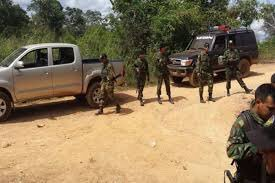
\includegraphics[width=300px]{72.jpg}%
\newline%
%
Caracas.{-} Al menos 16 personas se encuentran desaparecidas tras un supuesto enfrentamiento entre una banda armada y la guerrilla colombiana Ejército de Liberación Nacional (ELN) por el control de una mina ilegal de oro al sur del estado Bolívar.%
\newline%
%
La denuncia fue hecha por el disputado Américo de Grazia.  "Hubo un enfrentamiento (el domingo pasado) donde aparecen registrados 16 desaparecidos que se presume fallecieron asesinados en manos del ELN, entre ellos siete mujeres", dijo este martes en entrevista a Radio Caracas Radio, el parlamentario opositor.%
\newline%
%
Según el diputado, el enfrentamiento, que ocurrió en la mina El Candado, en la zona de Bochinche del estado Bolívar, dejó también seis heridos de bala, que escaparon y fueron atendidos en un hospital de Tumeremo, cerca de la mina.%
\newline%
%
El enfrentamiento supuestamente fue entre el ELN y la banda "El Coporo", controlada por un hombre apodado "El Tamao".%
\newline%
%
La zona del enfrentamiento colinda con Brasil, sin embargo, pobladores aseguran que el ELN ingresó a ese territorio a través del vecino estado Amazonas, fronterizo con Colombia. Las autoridades no han confirmado la presencia de esa guerrilla en Bolívar.%
\newline%
%
Periodistas de Bolívar aseguran que una comisión del Servicio Bolivariano de Inteligencia (Sebin), la Guardia Nacional, el Ejército, la Dirección General de Contrainteligencia Militar (Dgcim), y el Cuerpo de Investigaciones Científicas, Penales y Criminalísticas (Cicpc), fueron este martes a la mina para investigar lo ocurrido.%
\newline%
%
Los familiares de los desaparecidos protestaron el lunes y este martes en la entrada de la vía que conduce a la mina, para exigir a las autoridades que les informen qué ocurrió, según reportes de la prensa local.%
\newline%
%
Según videos que difundieron el diputado y habitantes de Tumeremo, dos helicópteros militares sobrevolaron la zona este martes.%
\newline%
%
"Helicóptero militar sobrevuela Tumeremo tras incursión y masacre del ELN en el Arco Minero", escribió en Twitter Rocío San Miguel, presidenta de la ONG Control Ciudadano, especializada en asuntos militares.%
\newline%
%
Tumeremo fue conmocionado en marzo de 2016 por la matanza a balazos de 17 mineros, cuyos cuerpos fueron localizados en una fosa común.%
\newline%
%
Otra masacre de 11 personas fue denunciada allí meses después.\newline%
\newline%
El 10 de febrero de este año, una incursión militar en una mina de la localidad de Guasipati, también en el estado Bolívar, dejó 18 muertos en lo que organizaciones de derechos humanos y dirigentes opositores calificaron de "masacre".%
\newline%
%
Tumeremo y Guasipati, regiones fronterizas con Brasil, forman parte del Arco Minero del Orinoco, extenso territorio que el Gobierno explota con compañías multinacionales para compensar la caída de los ingresos petroleros en medio de una grave crisis.%
\newline%
%
El 24 de agosto de 2017, ocho personas murieron en un choque entre presuntos delincuentes y militares en El Callao, también en Bolívar.%
\newline%
%
\end{document}